\documentclass{beamer}

%style
\mode<presentation>{
	\usetheme{goettingen}
}
%packages
\usepackage[utf8]{inputenc}
\usepackage[ngerman]{babel}
\usepackage{graphicx}

%Einstellungen Präsentation
\title{Verzögerte Differentialgleichungen}
\author{Raphael Unterer}
\institute{Mathematisches Seminar 2018}
\date{07.05.2018}

%Bilder
\graphicspath{{Pictures/}}

%Beginn der Präsentation
\begin{document}

%Titelseite
\begin{frame}
\titlepage
\end{frame}

%Inhaltsverzeichnis
\begin{frame}
\frametitle{Inhalt}
\tableofcontents
\end{frame}

\section{ENSO}

\subsection{El Niño Phänomen}
\begin{frame}
	\frametitle{El Niño Phänomen}
	\begin{itemize}
		\item[] Normale Situation
		\begin{figure}
			\includegraphics[width=0.7\linewidth, height=0.3\textheight]{ElNinoMap_Normal.png}
		\end{figure}
		\pause
		\item[] El Niño
		\begin{figure}
			\includegraphics[width=0.7\linewidth, height=0.3\textheight]{ElNinoMapElNino.png}
		\end{figure}
	\end{itemize}
\end{frame}

\subsection{Vezögerte Differentialgleichung (DDE)} 
\begin{frame}
	\frametitle{Verzögerte Differentialgleichung}
	\begin{itemize}
		\item[] Kelvin- und Rossby-Wellen
		\begin{figure}
			\includegraphics[width=0.7\linewidth, height=0.3\textheight]{ElNinoMap.png}
		\end{figure}
		\pause
		\item[] Verzögerte Differentialgleichung:
		\begin{equation}
			\dot{T}(t)=-cT(t)+aT(t-\frac{1}{2}\tau_K)-bT(t-(\frac{1}{2}\tau_R+\tau_K))-\epsilon(T(t))^3
		\end{equation}
	\end{itemize}
\end{frame}

\section{Analytische Lösung}

\subsection{Schrittweises Lösen}
\begin{frame}
	\frametitle{Schrittweises Lösen einer DDE}
	\begin{itemize}
		\item[] Beispiel
			\begin{equation}
			\dot{y}(t)=ky(t-\tau)=-y(t-1)
			\end{equation} 
			\pause
		\item[] Anfangsbedingung
			\begin{equation}
			y(t)=1 \textrm{ if }	-1\le t<0
			\end{equation}
			\pause
		\item[] Lösung im Bereich von 0 bis 1 
		 	\pause
		 	\begin{equation}
		 	\dot{y}=-1 \textrm{   daraus folgt  } y=1-t
		 	\end{equation} 	
	\end{itemize}
\end{frame}

\subsection{Charakteristische Gleichung}
\begin{frame}
\frametitle{Charakteristische Gleichung}
\begin{itemize}
	\item[] Beispiel
	\begin{equation}
	\dot{y}(t)=ky(t-\tau)
	\end{equation} 
	\item[] Ansatz
	\begin{equation}
	y(t) = ce^{\lambda t}
	\end{equation}
	\pause
	\item[] Einsetzen
	\begin{equation}
	\lambda ce^{\lambda t} = kce^{\lambda (t-\tau )}
	\end{equation} 	
	\pause
	\item[] Vereinfachen
	\begin{equation}
	\lambda  - ke^{-\lambda}= 0
	\end{equation}
\end{itemize}
\end{frame}

\section{Numerische Lösung}

\subsection{Chaotisches Verhalten}
\begin{frame}
	\frametitle{Chaotisches Verhalten ohne Dämpfungsterm}
	\begin{itemize}
		\item[] Gleichung ohne Dämpfung
			\begin{equation}
				\dot{T}(t)=-cT(t)+aT(t-\frac{1}{2}\tau_K)-bT(t-(\frac{1}{2}\tau_R+\tau_K))
			\end{equation}
			\pause
		\item[] Änderung des Parameters a
			\begin{figure}
				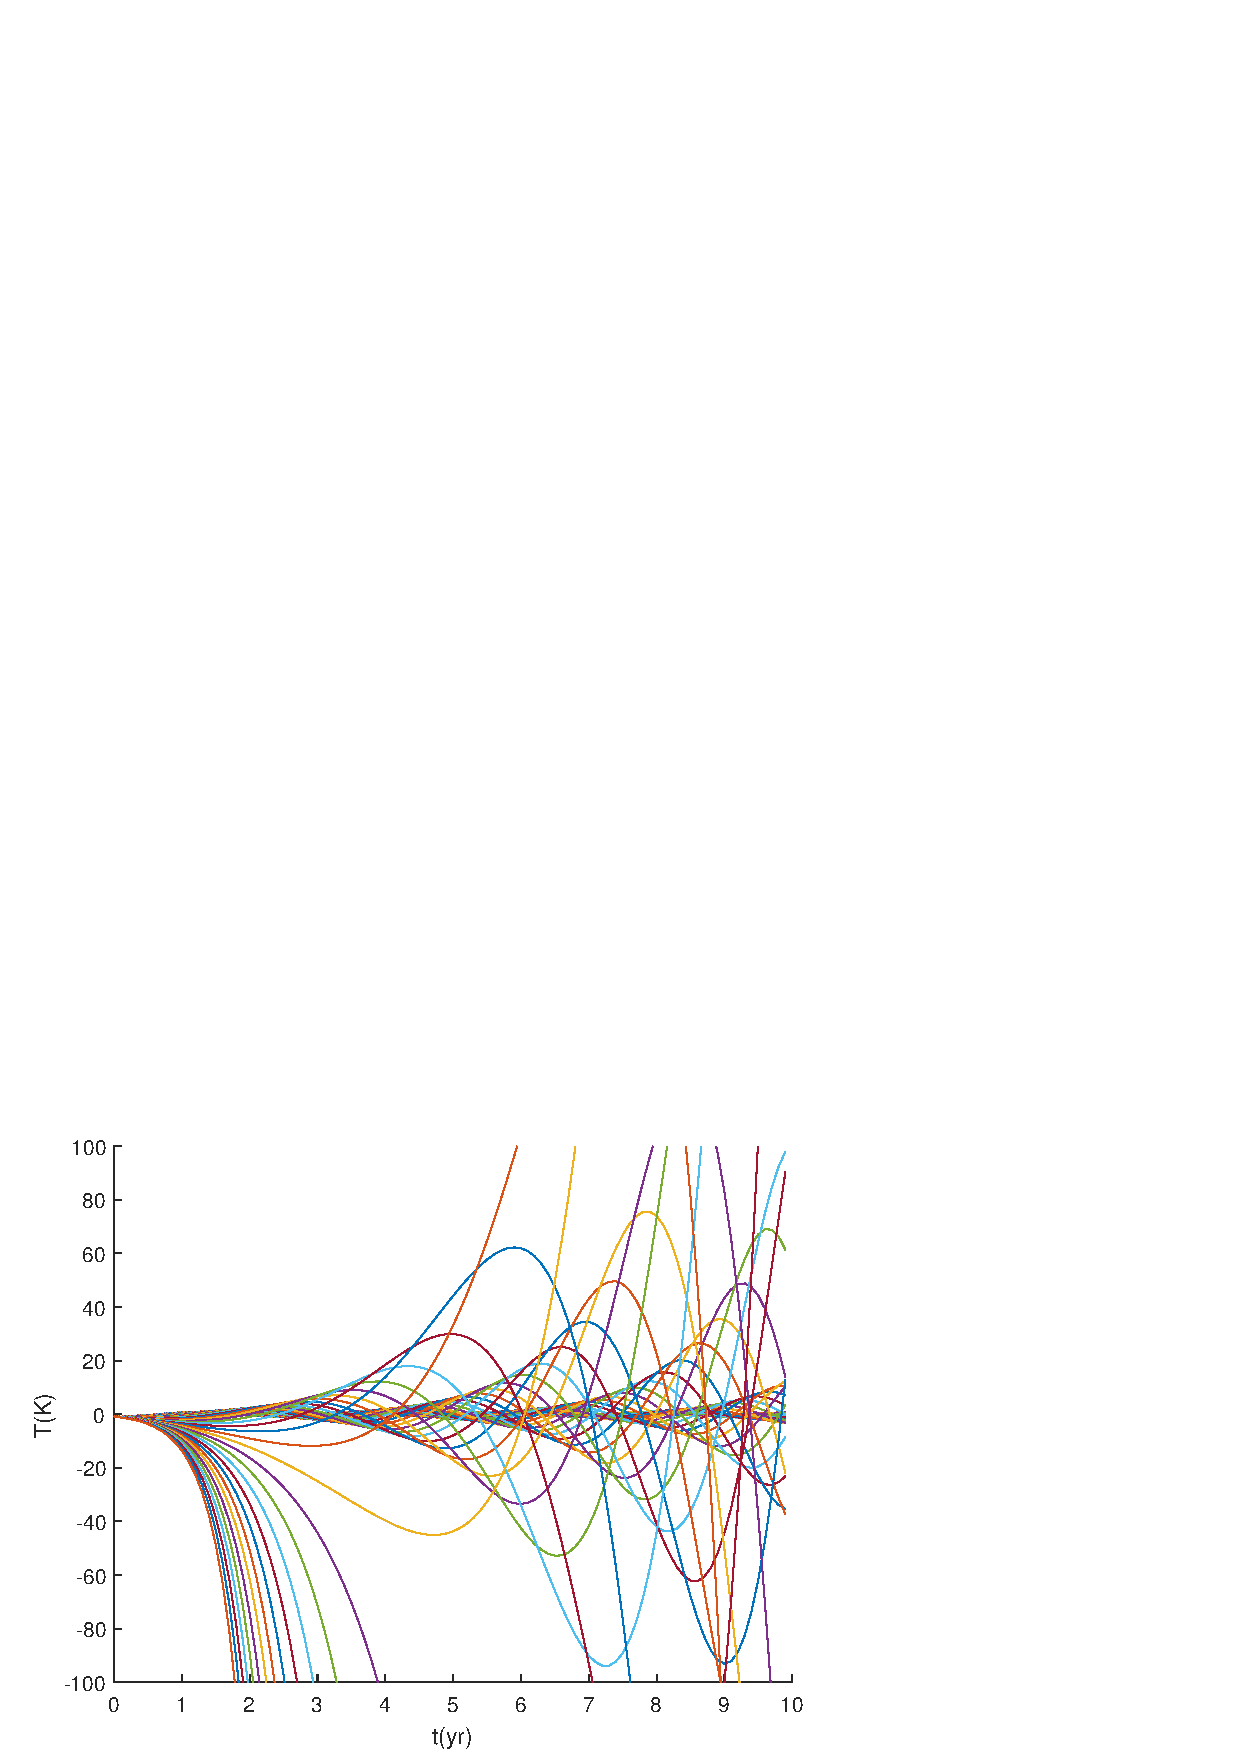
\includegraphics[width=0.9\linewidth, height=0.6\textheight]{param_a_e0.png}
			\end{figure}
	\end{itemize}
\end{frame}

\subsection{Vollständige Lösung}
\begin{frame}
\frametitle{Verhalten mit Dämpfungsterm}
\begin{itemize}
	\item[] Gleichung mit Dämpfung
	\begin{equation}
	\dot{T}(t)=-cT(t)+aT(t-\frac{1}{2}\tau_K)-bT(t-(\frac{1}{2}\tau_R+\tau_K))-\epsilon(T(t))^3
	\end{equation}
	\pause
	\item[] Änderung des Parameters a
	\begin{figure}
		\includegraphics[width=0.9\linewidth, height=0.6\textheight]{param_a.png}
	\end{figure}
\end{itemize}
\end{frame}

\subsection{Simulation}
\begin{frame}
\frametitle{Simulation und Vergleich mit realen Daten}
\begin{itemize}
	\item[] 
	\begin{figure}
		\includegraphics[width=0.9\linewidth, height=0.6\textheight]{simulation_95_98.png}
	\end{figure}
	\item[] Anfangswertvektor und Vergleichsdaten von \url{http://www.cpc.ncep.noaa.gov/data/indices/sstoi.indices}
\end{itemize}
\end{frame}

\end{document}